\chapter{Cross Plattform Frameworks}
\label{chap:CrossPlattformFrameworks}

Für die Realisierung eine Source-to-Source Compilers gibt es zwei relevante Faktoren,  die für die Realisierung ausschlaggebend sind.  Zum einen die Programmiersprachen in dem die beiden Frameworks entwickelt werden,  da bei der Übersetzung eine Brücke zwischen Quell und Zielsprache geschlagen werden muss.  Neben der Programmiersprache ist jedoch auch die Arbeitsweise eines Frameworks von essentieller Bedeutung.  Wie die Definition von Compilern bereits einführte,  müssen die Programme vor und nach der Übersetzung gleichwertig sein.  Dies implementiert,  dass das Verhalten der übersetzten Anwendungen nach der Übersetzung identisch seien muss wie das der Ursprungsanwendung.  Es ist also notwendig,  neben den sprachlichen auch die technischen Unterschiede zwischen den Frameworks zu kennen und diese im Rahmen der Kompilierung zu optimieren. 

\section{Frameworks}
Xamarin is eine Open Source-Plattform für das Erstellen mobiler Anwendungen für iOS und Android mit Hilfe des .NET Frameworks, welches von Microsoft weiterentwickelt wird.  Dabei ist Xamarin ist eine Abstraktionsebene, die die Kommunikation zwischen Code und dem zugrunde liegenden Plattformcode verwaltet.  Xamarin wird in einer verwalteten Umgebung ausgeführt, die Vorteile wie Speicherbelegung und Garbage Collection bietet.  Bei Xamarin.Forms handelt es sich um ein Open-Source-Benutzeroberflächenframework., mit dessen Hilfe Entwickler iOS- und Android- Anwendungen aus einer einzigen CodeBase erstellen können.  Dabei wird auf die in der .NET Welt bekannten Technologien XAML  für die Benutzeroberfläche und C\# für die Anwendungslogik zurückgegriffen.  Die einzelnen Benutzeroberflächen werden von Xamarin.Forms als native Steuerelemente auf jeder Plattform gerendert.  \footcite[Vgl.][Abgerufen am \today]{MicrosoftWhatIsXam2020}

Flutter ist ebenfalls wie Xamarin.Forms ein Open Source Framework für die Erstellung von 2D mobilen Anwendungen.  Dabei werden im Vergleich zu Xamarin.Forms keine nativen Steuerelemente für jede Plattform gerendert sondern beinhaltet eine Sammlung von so genannten Widgets, die von dem Framework vewaltet und gerendert werden.  Für die Anzeige dieser Widgets wird auf die 2D engine Skia zugegriffen.  Flutter geht diesen Weg,  da das Endergebnis der Anwendungen eine höhere Qualität verspricht, da die nativen Steuerelemente in Bezug auf Flexibilität und Qualität begrenzt sind.  Außerdem ist es durch die Verwendung derselben Renderes einfacher, von derselben Codebasis aus für mehrere Plattformen zu veröffentlichen,  ohne eine sorgfältige und kostspielige Planung vornehmen zu müssen,  um verschiedene Funktionssätze und API-Merkmale aufeinander abzustimmen.\footcite[Vgl.][Abgerufen am \today]{GoogleFlutterFAQ2020}

Dieser essentielle Unterschied zwischen den Frameworks werden in den folgenden Abschnitten dieser Arbeit deutlicher und sind bei der Übersetzung der Anwendungen fokussiert zu Berücksichtigen. 
\subsection{Projekte}
Xamarin.Forms Projektmappen setzen sich aus mehreren Projekten zusammen., jeweils eins für die Plattform (iOS/ Android),  welche den plattformspezifischen Code und assets in Form von Icons und Metadaten beinhalten sowie ein zusätzliches für den Quelltext,  der zwischen den Plattformen geteilt wird.  \footcite[Vgl.][S. 25f.]{Petzold2016} Im Gegensatz dazu gibt es bei Flutter nur ein Projekt, welches alle notwendigen Inhalte für iOS und Android beinhaltet.  Für plattformspezifischen Code gibt es jeweils einen Ordner für iOS und Android. \footcite[Vgl.][S. 113]{Biessek2019}

\subsection{Views}
Views (zu Deutsch Ansichten) sind visuelle Elemente die in zwei Kategorien unterschieden werden können.  Controls, die für die Sammlung von Benutzereingaben oder die Ausgabe von Daten sind.  Sowie Layouts die eine Sammlung von Ansichten beinhalten und für die Anordnung der untergeorderten Ansichten in der Benutzeroberfläche verantwortlich sind.  Außerdem arbeitet sie mit jeder untergeordneten Ansicht zusammen, um die endgültige Rendering-Größe zu bestimmen.\footcite[Vgl.][Abgerufen am \today]{Ritscher2020}
\subsubsection{Pages}
Pages (zu Deutsch: Ansichtseiten) sind visuelle Elemente einer Anwendung die den gesamten Bildschirm belegen und zu den Layout Views gehören.  Xamarin Forms bietet dafür 
verschiedene Alternativen an,  die in \ref{fig:Xamarin.Forms Pages} grafisch dargestellt sind.\footcite[Vgl.][Abgerufen am \today]{MicrosoftXamPages2016}

\begin{figure}[!ht]
 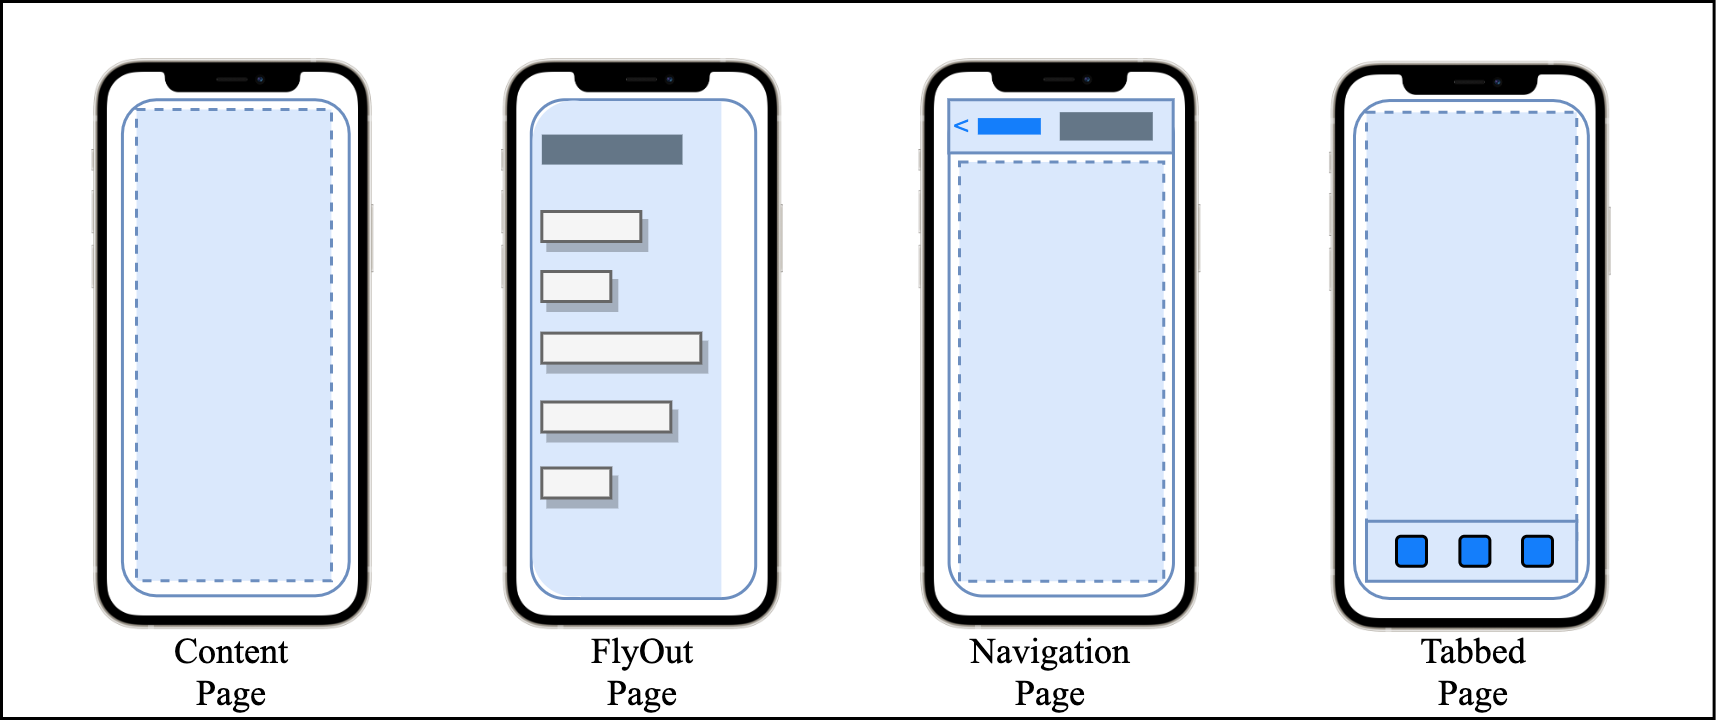
\includegraphics[width=\textwidth,height=\textheight,keepaspectratio]{Images/CrossPlattformFrameworks/XamarinFormsPages.png}
 \caption[Xamarin.Forms Pages]{Xamarin.Forms Pages\footnotemark}
 \label{fig:Xamarin.Forms Pages}
\end{figure}
\footcitetext[Abbildung in Anlehnung an ][Abgerufen am \today]{MicrosoftXamPages2016}
Wie die Darstellung präsentiert, hat die Auswahl einer Page einen direkten Einfluss auf das Navigationskonzept innerhalb der Anwendung.  Abgesehen von der ContentPage, die ausschließlich eine View anzeigt haben die jeweiligen Seiten das folgende Navigationskonzept: \footcite[Vgl.][Abgerufen am \today]{MicrosoftXamPages2016}

\begin{itemize}
\setlength\itemsep{-0.6em}
 \item FlyOutPage: Eine Seite, die zwei Bereiche für die Seite hat. Typischerweise enthält das Flyout ein Menü über welches zwischen den eigentlichen Inhaltsseiten navigiert werden kann.
 \item NavigationPage: Eine Seite,  die eine Navigationsleiste enthält.  Die Seiten werden auf einem Stapel gehalten und es kann zwischen ihnen gesprungen werden.  Die Navigationsleiste kann sowohl Navigationsschaltflächen als auch einen Titel enthalten.
 \item TabbedPage: Eine Container-Seite.  Die TabbedPage fungiert als Container,  der die mit jeder Registerkarte verbundenen Inhaltsseiten enthält.
\end{itemize}

Die Auswahl einer Page wird innerhalb des Wurzelknoten der XAML Datei definiert.  Dies wird in Quelltext \ref{lst:TabbedPage} dargestellt. 

\begin{minipage}{\linewidth}
\lstinputlisting[label={lst:TabbedPage},caption={Xamarin.Forms TabbedPage definition}, language=XML]{SourceCode/XamarinFormsTabbedPage.XAML}
\end{minipage}

Das Beispiel zeigt eine TabbedPage mit drei in diesem Falle leeren NavigationsPages die als Children der TabbedPage hinzugefügt werden.  Im Gegensatz zu der TabbedPage hat die FlyoutPage keine Sammlung von ChildrenPages sondern ein sogenanntes "Flyout" welches das Menu beinhaltet und die entsprechend ausgewählte Seite in eine Detailansicht läd.  Dies wird in Quelltext \ref{lst:FlyOutPage} dargestellt.

\begin{minipage}{\linewidth}
\lstinputlisting[label={lst:FlyOutPage},caption={Xamarin.Forms FlyOut definition}, language=XML]{SourceCode/XamarinFormsFlyoutPage.XAML}
\end{minipage}

Im Gegensatz zu Xamarin.Forms lässt sich bei Flutter auf der Ebene der Wurzel kein Navigationskonzept definieren,  sondern ausschließlich das Style der Anwendung.  Flutter unterstützt drei alternativen: MaterialApp erzeugt eine App mit dem von Google entwickelten Material Design, CupertinoApp für eine App im iOS-Stil oder die Definition eines eigenen Styles für eine individuelle Anzeige.  \footcite[Vgl.][Abgerufen am \today]{GoogleFlutterPages2020}  Quelltext \ref{lst:MaterialApp} zeigt die Definition einer MaterialDesign App in Flutter.

\begin{minipage}{\linewidth}
\lstinputlisting[label={lst:MaterialApp},caption={Flutter MaterialApp definition}, language=Dart]{SourceCode/MaterialApp.Dart}
\end{minipage}

Von diesem Widget aus ist die eigentliche erste Seite ein weiteres zustandsabhängiges Widget.  Dieses besteht aus zwei Teilen:  Der erste Teil, der selbst unveränderlich ist, erzeugt ein State-Objekt, das den Zustand des Objekts enthält.  Das State-Objekt bleibt während der Lebensdauer des Widgets bestehen. Das State-Objekt implementiert die build()-Methode für das zustandsabhängige Widget.  Wenn sich der Zustand des Widget-Baums ändert,  wird setState() aufgerufen was einen Build des entsprechenden Teils der Benutzeroberfläche auslöst.  In Flutter ist die Benutzeroberfläche (auch bekannt als Widget-Baum) unveränderlich,  dass bedeutet da der Zustand nicht mehr geändert werden kann, sobald dieser aufgebaut ist.  Sie ändern Felder in Ihrer State-Klasse und rufen dann setState() auf, um den gesamten Widget-Baum neu zu erstellen. \footcite[Vgl.][Abgerufen am \today]{GoogleFlutterSharedPreferences2020} 

Damit die Navigation ähnlich wie in Xamarin.Forms definiert werden kann müssen verschiedene Widgets in einem Widget Baum verschachtelt werden.  Quelltext \ref{lst:FlutterTabbedApp} zeigt dies für die Arbeit mit Tabbs.  In diesem Beispiel wird eine TabBar mit drei Tab-Widgets erstellt und diese innerhalb einer AppBar platziert.\footcite[Vgl.][Abgerufen am \today]{GoogleFlutterTabs2020} 


\begin{minipage}{\linewidth}
\lstinputlisting[label={lst:FlutterTabbedApp},caption={Flutter Tab Layout definition}, language=Dart]{SourceCode/TabbedPage.Dart}
\end{minipage}

\subsubsection{Layouts}

Layouts werden in Xamarin.Forms verwendet, um die Steuerelemente der Benutzeroberfläche zu visuellen Strukturen zusammenzustellen.  Dabei unterscheidet man zwischen Layouts die ausschließlich einen oder mehrere Inhalte beinhalten können.  Xamarin.Forms bietet eine vielzahl von Layouts an die in \ref{fig:Xamarin.Forms Layouts} grafisch dargestellt werden.

\begin{figure}[!ht]
 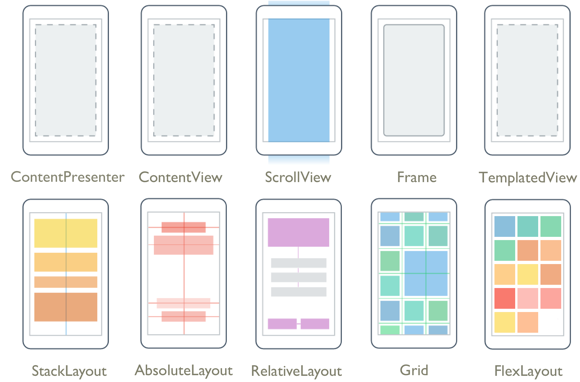
\includegraphics[width=\textwidth,height=\textheight,keepaspectratio]{Images/CrossPlattformFrameworks/XamarinFormsLayouts.png}
 \caption[Xamarin.Forms Layouts]{Xamarin.Forms Layouts\footnotemark}
 \label{fig:Xamarin.Forms Layouts}
\end{figure}
\footcitetext[Abbildung in Anlehnung an ][Abgerufen am \today]{MicrosoftXamLayouts2018}

An dieser Stelle ist es nun wichtig zu analysieren,  wie man jedes Xamarin.Forms Layout in Flutter nachbilden kann.  Dafür wird folgend die Funktion der einzelnen Layouts anhand der Xamarin.Forms Dokumentation\footcite[Vgl.][Abgerufen am \today]{MicrosoftXamLayouts2018} erklärt und ein Flutter Layout mit den gleichen Eigenschaften herausgestellt. 

\begin{itemize}
\setlength\itemsep{-0.6em}
 \item ContentView: ContentView enthält ein einzelnes untergeordnetes Element, das mit der Eigenschaft "Content" festgelegt wird. Die Eigenschaft Content kann auf jedes View-Derivat gesetzt werden, auch auf andere Layout-Derivate. ContentView wird meist als Strukturelement verwendet und dient als Basisklasse zu Frame.
 \item Frame: Die Klasse Frame leitet sich von ContentView ab und zeigt einen Rahmen um die Ansicht.  In Flutter kann auf das BoxDecoration widget zugegriffen werden es beschreibt, wie ein Kasten auf dem Bildschirm dargestellt werden soll, und kann als Rahmen dargestellt werden. \footcite[Vgl.][Abgerufen am \today]{GoogleFlutterBoxDecoration2020}
  \item ScrollView: Ist in der Lage, seinen Inhalt zu scrollen.  Die Eigenschaft Content auf eine Ansicht oder ein Layout fest, das zu groß ist, um auf den Bildschirm zu passen.  Legen Sie die Eigenschaft Orientierung fest, um anzugeben, ob der Bildlauf vertikal, horizontal oder beides sein soll. In Flutter ist die nächste Entsprechung das SingleChildScrollView-Widget.\footcite[Vgl.][Abgerufen am \today]{GoogleFlutterSingleChildScrollView2020}
   \item StackLayout: Positioniert untergeordnete Elemente in einem Stapel entweder horizontal oder vertikal,  basierend auf der Eigenschaft Orientation.  Flutter hat ein ähnliches Konzept, anstatt der Orientation werden Kinder durch die Widgets Row und Column vertical oder horizontal ausgerichtet. 
 \item Grid: Grid positioniert seine untergeordneten Elemente in einem Raster aus Zeilen und Spalten. Die Position eines untergeordneten Elements wird über die angehängten Eigenschaften Row, Column, RowSpan und ColumnSpan angegeben.  Außerdem wird das Grid Control häufig verwendet um Steuerelemente zu stapeln.  Das nächste Äquivalent zu einem Grid wäre ein GridView. Dieses ist viel leistungsfähiger als das, was Sie in Xamarin.Forms gewohnt sind. Ein GridView bietet einen automatischen Bildlauf, wenn der Inhalt den sichtbaren Bereich überschreitet. \footcite[Vgl.][Abgerufen am \today]{GoogleFlutterGridView2020}  Für das Stapeln von Elementen,  in Flutter lässt sich dies mit dem Stack-Widget erreichen.  \footcite[Vgl.][Abgerufen am \today]{GoogleFlutterStack2020}
 \item AbsolutLayout: Positioniert untergeordnete Elemente an bestimmten Positionen relativ zu ihrem übergeordneten Element. Die Position eines untergeordneten Elements wird über die angehängten Eigenschaften LayoutBounds und LayoutFlags angegeben. Ein AbsoluteLayout ist nützlich, um die Positionen von Ansichten zu animieren.
 \item RelativeLayout:  Positioniert untergeordnete Elemente relativ zum RelativeLayout selbst oder zu ihren Geschwistern. Die Position eines Kindelements wird über die angehängten Eigenschaften angegeben, die auf Objekte vom Typ Constraint und BoundsConstraint gesetzt werden.
\end{itemize}

\subsubsection{Steuerelemente}

Xamarin.Forms-Ansichten sind die Bausteine von plattformübergreifenden mobilen Benutzeroberflächen. Ansichten sind Objekte der Benutzeroberfläche wie Beschriftungen, Schaltflächen und Schieberegler, die in anderen grafischen Programmierumgebungen üblicherweise als Steuerelemente oder Widgets bezeichnet werden. Die von Xamarin.Forms unterstützten Ansichten leiten sich alle von der Klasse View ab. \footcite[Vgl.][Abgerufen am \today]{MicrosoftXamViews2020}

\subsubsection{Steuerelemente für die Darstellung}
Steuerelemente für die Darstellung sind Elemente die neben der Darstellung und der Benutzerfahrung keine weitere Funktionalität haben. Klassischerweise zeigen diese Informationen die für die Arbeit mit der Anwendung wichtig sind an.  Die folgende Aufzählung zeigt die wichtigsten Steuerelemente aus Xamarin.Forms für die Darstellung, \footcite[Vgl.][Abgerufen am \today]{MicrosoftXamLayouts2018} wobei zu zeichnende Elemente wie die Ellipse,  eine Linie,  Path,  Polygon, Polyline und Rectangle nicht besonders aufgeführt werden, da diese bei Flutter einfach auf das Canvas gezeichnet werden können.  \footcite[Vgl.][Abgerufen am \today]{GoogleFlutterCanvas2020}

\begin{itemize}
\setlength\itemsep{-0.6em}
 \item BoxView zeigt in Xamarin.Forms ein einfarbiges Rechteck an. In der Praxis wird dieses Control auch häufig für die Darstellung von Seperatoren zwischen zwei Informationen verwendet.  Dafür wird in Xamarin.Forms die Höhe oder Breite des Controls auf 1 Pixel limitiert.  Für die Verwendung als seperator bietet Flutter das sogenannte Divider Widget an, welches überall verwendet werde kann um Content zu trennen.  Mit dem Widget SizedBox bietet Flutter jedoch auch ein Widget für die Zeichnung von Boxen mit einer gewissen Größe an.  \footcite[Vgl.][Abgerufen am \today]{GoogleFlutterSizedBox2020}
 \item Label zeigt einzeilige Textstrings oder mehrzeilige Textblöcke an, entweder mit konstanter oder variabler Formatierung. Für Label gibt es bei Flutter mehrere alternativen.  Das Text dem Xamarin.Forms Label am nahekommenste Widget ist "Text" was die Darstellung mit einem einzigen stil erlaubt. \footcite[Vgl.][Abgerufen am \today]{GoogleFlutterText2020} Ebenso bietet Flutter jedoch auch die Möglichkeit RichText in einem entsprechenden Widget anzuzeigen. \footcite[Vgl.][Abgerufen am \today]{GoogleFlutterRichText2020}
 \item Image zeigt ein Bitmap an, diese können über das Web heruntergeladen, als Ressourcen in über das gemeinsame Projekt oder in Plattformprojekte eingebettet  werden.  Flutter bietet ebenfalls ein Image Steuerelement an, welches die gleichen Quellen für Bilder unterstützt wie Xamarin.Forms. \footcite[Vgl.][Abgerufen am \today]{GoogleFlutterImage2020}
 \item Map zeigt eine Karte an.  Für Flutter gibt es mehrere Anbietet für Karten z.B. Leamaps und Google Maps, welches direkt von den Flutter Entwickelern angbeoten wird. \footcite[Vgl.][Abgerufen am \today]{GoogleFlutterMap2020}
 \item WebView zeigt Web-Seiten oder HTML-Inhalte an.  Das Widget "webview\_flutter" bietet eine entsprechende Implementierung für Flutter an. \footcite[Vgl.][Abgerufen am \today]{GoogleFlutterWebView2020}
\end{itemize}

\subsubsection{Steuerelemente die Aktionen auslösen}

Die folgenden Steuerelemente sind Elemente,  welche etwas in der mobilen Anwendung auslösen.  Diese Elemente benötigen eine Interaktion über Gesten des Anwenders mit der Anwendung. 
\begin{itemize}
\setlength\itemsep{-0.6em}
 \item Button ist ein rechteckiges Objekt, das Text anzeigt und ein Clicked-Ereignis auslöst, wenn es gedrückt wurde.  Flutter bietet eine Vielzahl von Buttons an, wobei der "FlatButton" dem Xamarin.Forms button am nähesten kommt.
 \item ImageButton ist ein rechteckiges Objekt, das ein Bild anzeigt und ein Clicked-Ereignis auslöst, wenn es gedrückt wurde.  In Flutter stehen dafür der IconButton zur Verfügung.
  \item RadioButton erlaubt die Auswahl einer Option aus einer Menge und feuert ein CheckedChanged-Ereignis, wenn die Auswahl erfolgt. Flutter bietet genau wie Xamarin.Forms einen RadioButton an,  mit identischer Arbeitsweise
 \item RefreshView ist ein Container-Steuerelement, das eine Pull\-to\-Refresh-Funktionalität für scrollbare Inhalte bietet.  Das Widget "pull\_to\_refresh" bietet ähnlich wie die Xamarin.Forms alternative an durch herunterziehen des Contents eine Aktion auszulösen.
 \item SearchBar zeigt einen Bereich an, in dem der Benutzer eine Textzeichenfolge eingeben kann, sowie eine Schaltfläche (oder eine Tastaturtaste), die der Anwendung signalisiert, eine Suche durchzuführen. Das Widget "flutter\_search\_bar" bietet die Möglichkeit den Inhalt zu Filtern.  Jedoch kann es nicht wie bei Xamarin.Forms frei platziert werden, sondern wird im Rahmen der Navigationsleiste abgebildet. 
 \item SwipeView ist ein Container-Steuerelement, das sich um ein Inhaltselement legt und Kontextmenüelemente bereitstellt, die durch eine Wischgeste angezeigt werden.  Flutter selber bietet kein Widget mit dieser Funktionalität an.  Für Listen steht jedoch mit "flutter\_slidable" ein OpenSource Widget zur Verfügung. 
\end{itemize}



\subsubsection{Steuerelemente um Werte zu setzen}

Steuerelemente die Werte setzen sind User Interface Elemente die von einem Anwender durch Interaktion mit Werten versehen werden können um diese in der Anwendung zu verarbeiten.  In diesem Unterabschnitt wird nicht auf Elemente eingegangen,  die zur Eingabe und Manipulation von Texten zur Verfügung stehen, da diesen Steuerelementen ein eigener Unterabschnitt gewährt wird.  Xamarin.Forms bietet eine Vielzahl von Steuerelementen, die an dieser Stelle aufgeführt werden. Zusätzlich wird wie in den vorherigen Abschnitten erläutert, wie dieses Verhalten bei Flutter generiert werden kann. 
\begin{itemize}
\setlength\itemsep{-0.6em}
 \item CheckBox ermöglicht dem Benutzer die Auswahl eines booleschen Wertes mit Hilfe einer Art Schaltfläche, die entweder markiert oder leer sein kann. Flutter bietet ebenfalls ein Checkbox Control an,  das Material Design Checkbox. 
  \item Switch hat die Form eines Ein/Aus-Schalters, damit der Benutzer einen booleschen Wert auswählen kann, für das es ebenfalls eine entsprechendes Flutter Widget gibt. 
 \item Slider bieten Benutzern die Option einen  Wert aus einem kontinuierlichen Bereich auswählen, der mit den Eigenschaften Minimum und Maximum festgelegt wurde.  Flutter bietet ebenfalls ein Widget für Slider an
 \item Stepper ermöglicht es dem Benutzer, einen doppelten Wert aus einem Bereich von inkrementellen Werten auszuwählen, die mit den Eigenschaften Minimum, Maximum und Inkrement festgelegt wurden.  Von Haus aus gibt es bei Flutter kein Steuerelement,  welches ähnliche Eigenschaften anbietet.  Die Open Source Community hat mit dem number\_inc\_dec Plugin aber eine Widget entwickelt welches wie die Xamarin.Forms alternative arbeitet. 
 \item DatePicker ermöglicht es dem Benutzer, ein Datum mit der Datumsauswahl der Plattform auszuwählen.  In Flutter stehen dafür kein Widget sondern eine Funktion zur Verfügung,  die klassischerweise, wie in Quelltext , in einem Gesture Detector auf einem anderen Widget ausgeführt wird.  
 \item TimePicker ermöglicht dem Benutzer die Auswahl einer Zeit mit dem spezifischen TimePicker der Plattform.  Wird ähnlich wie der Datepicker nicht als Widget sonders als Funktionalität ausgeliefert,  ein mögliche Definition ist in Quelltext \ref{lst:FlutterTimePicker} dargestellt.
 
 \begin{minipage}{\linewidth}
\lstinputlisting[label={lst:FlutterTimePicker},caption={Verwendung von Timepickern in Flutter}, language=Dart]{SourceCode/FlutterTimePicker.Dart}
\end{minipage}

\end{itemize}

\subsubsection{Steuerelemente um Text zu manipulieren}
Wie bereits im vorherigen Abschnitt beschrieben sind Steuerelemente zur Eingabe und manipulation von Texten Strang genommen ebenfalls Steuerelemente zum setzen von Werten.  In Xamarin Forms stehen die folgenden beiden Steuerelemente für die Arbeit mit Texten zur Verfügung:
\begin{itemize}
\setlength\itemsep{-0.6em}
 \item Entry ermöglicht dem Benutzer die Eingabe und Bearbeitung einer einzelnen Textzeile., optional kann dieses als Passworteingabe mit Sternen maskiert werden.
 \item Editor ermöglicht dem Benutzer die Eingabe und Bearbeitung mehrerer Textzeilen
\end{itemize}

In flutter gibt es ausschließlich das Textfield Widget, welches die Funktionalitäten von beiden Xamarin.Forms controlls bündelt.  Standardmäßig bietet das TextField Widget die Eingabemöglichkeit für eine Zeile ähnlich wie das Entry Steuerelement kann aber durch die Eigenschaft "keyboardType: TextInputType.multiline" wie ein entry fungieren wobei optional auch eine Anzahl von maximalen Zeilen übergeben werden kann.  Dies wird in Quelltext dargestellt.

 \begin{minipage}{\linewidth}
\lstinputlisting[label={lst:FlutterTextField},caption={TextField mit mehreren Zeilen in Flutter}, language=Dart]{SourceCode/FlutterTextField.Dart}
\end{minipage}


\subsubsection{Steuerelemente um eine Aktivität anzudeuten}

In mobilen Anwendungen kann es aufgrund der Limitierten Hardware Ressourcen und der begrenzten Netzwerkanbindung dazu kommen, dass Aktionen etwas länger dauern,  als es der Anwender erwarten würden.  Dafür stehen in Xamarin.Forms Steuerelemente zur Verfügung, die dem Anwender das Andauern einer Aktivität andeuten.  Die folgenden Elemente stehen Xamarin.Forms Entwicklern zur Verfügung:

\begin{itemize}
\setlength\itemsep{-0.6em}
 \item ActivityIndicator verwendet eine Animation, um zu zeigen, dass die Anwendung eine langwierige Aktivität ausführt, ohne einen Hinweis auf den Fortschritt zu geben.  Für Flutter Anwendungen steht ein ähnliches Widget zur Verfügung das als "CircularProgressIndicator" bezeichnet wird. 
 \item ProgressBar verwendet eine Animation, um zu zeigen, dass die Anwendung durch eine langwierige Aktivität fortschreitet. In Flutter steht mit dem "LinearProgressIndicator" Widget ebenfalls eine Progressbar zur Verfügung.
\end{itemize}

\subsubsection{Steuerelemente um Sammlungen anzuzeigen}

Bei diesen Steuerelementen handelt es sich um Elemente, die zur Anzeige von Daten-Sammlungen spezialisiert sind.  Xamarin.Forms stellt die folgenden Steuelemente zur Verfügung.

\begin{itemize}
\setlength\itemsep{-0.6em}
 \item CarouselView zeigt eine blätterbare Liste von Datenelementen an.  Für Flutter steht ein ähnliches Widget mit dem "carousel\_slider" zur erfügung
 \item IndicatorView zeigt Indikatoren an, die die Anzahl der Elemente in einer CarouselView darstellen
 \item Picker zeigt ein ausgewähltes Element aus einer Liste von Textzeichenfolgen an und ermöglicht die Auswahl dieses Elements, wenn die Ansicht angetippt wird.  Das Picker Widget ist bereits wie im Date,- und Time-Picker beschrieben kein Controll sondern eine Funktion, welches durch Gesten auf andere Widges ausgeführt werden kann. 
 \item TableView zeigt eine Liste von Zeilen mit optionalen Überschriften und Unterüberschriften an.  Das äquivalente flutter- Widget ist als Table Verfügbar.
\end{itemize}

\subsubsection{Listen}

Listen sind ebenfalls Steuerelemente für die Anzeige und Interaktion mit Sammlungen,  bekommen jedoch wegen ihrer häufigen Verwendung einen eigenen Abschnitt. In Xamarin.Form existieren ein Listview und ein CollectionView Control,  wobei zweiteres eine optimierung der Listview ist.  Das Äquivalent zu einer ListView in Flutter ist ... eine ListView!

In einer Xamarin.Forms ListView erstellen Sie eine ViewCell und möglicherweise einen DataTemplateSelector und übergeben diese an die ListView, die jede Zeile mit dem rendert, was Ihr DataTemplateSelector oder ViewCell zurückgibt. Allerdings müssen Sie oft darauf achten, dass Sie Cell Recycling einschalten, da es sonst zu Speicherproblemen und langsamen Scrollgeschwindigkeiten kommen kann.Aufgrund des unveränderlichen Widget-Musters von Flutter übergeben Sie eine Liste von Widgets an Ihre ListView, und Flutter kümmert sich darum, dass das Scrollen schnell und reibungslos funktioniert

In Xamarin.Forms hat die ListView eine ItemTapped-Methode, um herauszufinden, welches Element angeklickt wurde. Es gibt viele andere Techniken, die Sie vielleicht verwendet haben, wie z. B. die Überprüfung, wenn sich das SelectedItem- oder EventToCommand-Verhalten ändert. In Flutter verwenden Sie die Touch-Behandlung, die von den übergebenen Widgets bereitgestellt wird.

Wenn Sie in Xamarin.Forms die ItemsSource-Eigenschaft an eine ObservableCollection gebunden haben, würden Sie einfach die Liste in Ihrem ViewModel aktualisieren. Alternativ könnten Sie der ItemSource-Eigenschaft auch eine neue Liste zuweisen. In Flutter funktionieren die Dinge ein wenig anders. Wenn Sie die Liste der Widgets innerhalb einer setState()-Methode aktualisieren, würden Sie schnell sehen, dass sich Ihre Daten visuell nicht geändert haben. Das liegt daran, dass die Flutter-Rendering-Engine beim Aufruf von setState() den Widget-Baum betrachtet, um zu sehen, ob sich etwas geändert hat. Wenn sie zu Ihrer ListView kommt, führt sie eine == Prüfung durch und stellt fest, dass die beiden ListViews gleich sind. Es hat sich nichts geändert, also ist keine Aktualisierung erforderlich. Eine einfache Möglichkeit, Ihre ListView zu aktualisieren, besteht darin, eine neue Liste innerhalb von setState() zu erstellen und die Daten aus der alten Liste in die neue Liste zu kopieren. Dieser Ansatz ist zwar einfach, aber für große Datensätze nicht zu empfehlen. Die empfohlene, effiziente und effektive Art, eine Liste zu erstellen, verwendet einen ListView.Builder. Diese Methode ist großartig, wenn Sie eine dynamische Liste oder eine Liste mit sehr großen Datenmengen haben. Dies ist im Wesentlichen das Äquivalent von RecyclerView unter Android, das automatisch Listenelemente für Sie recycelt:
Anstatt eine "ListView" zu erstellen, erstellen Sie einen ListView.builder, der zwei wichtige Parameter benötigt: die anfängliche Länge der Liste und eine ItemBuilder-Funktion. Die ItemBuilder-Funktion ähnelt der getView-Funktion in einem Android-Adapter; sie nimmt eine Position an und gibt die Zeile zurück, die an dieser Position gerendert werden soll. Schließlich, aber am wichtigsten, beachten Sie, dass die onTap()-Funktion die Liste nicht mehr neu erstellt, sondern ihr stattdessen etwas hinzufügt.



\subsubsection{Gesten}
In Xamarin.Forms können Elemente ein Klick-Ereignis enthalten, an das Sie anhängen können. Viele Elemente enthalten auch einen Befehl, der an dieses Ereignis gebunden ist. Alternativ dazu würden Sie den TapGestureRecognizer verwenden. In Flutter gibt es zwei sehr ähnliche Möglichkeiten: Wenn das Widget die Ereigniserkennung unterstützt, übergeben Sie ihm eine Funktion und behandeln es in der Funktion. Zum Beispiel hat der ElevatedButton einen onPressed-Parameter. Alternativ wenn das Widget keine Ereigniserkennung unterstützt, verpacken Sie das Widget in einen GestureDetector und übergeben Sie eine Funktion an den Parameter onTap.

In Xamarin.Forms würden Sie dem VisualElement einen GestureRecognizer hinzufügen. Normalerweise wären Sie auf TapGestureRecognizer, PinchGestureRecognizer und PanGestureRecognizer beschränkt, es sei denn, Sie haben einen eigenen erstellt. Flutter kann mit Hilfe des GestureDetectors deutlich mehr Gesten behandeln als Xamarin.Forms.

\subsubsection{Animation}
In Xamarin.Forms erstellen Sie einfache Animationen mit ViewExtensions, die Methoden wie FadeTo und TranslateTo enthalten. Sie würden diese Methoden in einer Ansicht verwenden, um die gewünschten Animationen auszuführen.

In Flutter animieren Sie Widgets mithilfe der Animationsbibliothek, indem Sie Widgets in ein animiertes Widget einwickeln. Verwenden Sie einen AnimationController, der eine Animation<double> ist, die die Animation pausieren, suchen, stoppen und umkehren kann. Er benötigt einen Ticker, der signalisiert, wenn vsync passiert, und erzeugt eine lineare Interpolation zwischen 0 und 1 auf jedem Frame, während er läuft. Anschließend erstellen Sie eine oder mehrere Animationen und hängen sie an den Controller.Zum Beispiel könnten Sie CurvedAnimation verwenden, um eine Animation entlang einer interpolierten Kurve zu implementieren. In diesem Sinne ist der Controller die "Master"-Quelle des Animationsverlaufs und die CurvedAnimation berechnet die Kurve, die die standardmäßige lineare Bewegung des Controllers ersetzt. Wie Widgets arbeiten auch Animationen in Flutter mit Komposition.
Beim Aufbau des Widget-Baums weisen Sie die Animation einer animierten Eigenschaft eines Widgets zu, z. B. der Deckkraft einer FadeTransition, und sagen dem Controller, dass er die Animation starten soll.

\subsection{Navigation}
In Xamarin.Forms bietet die Klasse NavigationPage eine hierarchische Navigation, bei der der Benutzer durch die Seiten, vorwärts und rückwärts, navigieren kann.

Flutter hat eine ähnliche Implementierung, die einen Navigator und Routen verwendet. Eine Route ist eine Abstraktion für eine Seite einer App, und ein Navigator ist ein Widget, das Routen verwaltet. Eine Route bildet grob eine Seite ab. Der Navigator arbeitet ähnlich wie die Xamarin.Forms NavigationPage, indem er Routen push() und pop() kann, je nachdem, ob man zu einer Ansicht hin oder von ihr zurück navigieren möchte.

\subsubsection{Navigation zu anderen Apps}
In Xamarin.Forms verwenden kann, um zu einer anderen Anwendung zu navigieren, ein bestimmtes URI-Schema verwendet werden.  So z.B. mit dem Befehl Device.OpenUrl("mailto://") das Standard E-Mail-Programm des Gerätes geöffnet werden verwenden.
Um diese Funktionalität in Flutter zu implementieren,  muss eine native Plattformintegration oder eine vorhandenes Plugin, wie z. B. urllauncher verwendet werden.  
\subsection{Async UI}
Dart hat ein Single-Thread-Ausführungsmodell mit Unterstützung für Isolates (eine Möglichkeit, Dart-Code in einem anderen Thread auszuführen), eine Ereignisschleife und asynchrone Programmierung. Sofern Sie kein Isolate erzeugen, wird Ihr Dart-Code im Haupt-Thread der Benutzeroberfläche ausgeführt und von einer Ereignisschleife gesteuert.

Das Single-Thread-Modell von Dart bedeutet nicht, dass Sie alles als blockierende Operation ausführen müssen, die das Einfrieren der Benutzeroberfläche verursacht. Ähnlich wie bei Xamarin.Forms müssen Sie den UI-Thread frei halten. Sie würden async/await verwenden, um Aufgaben auszuführen, bei denen Sie auf die Antwort warten müssen.

In Flutter verwenden Sie die asynchronen Möglichkeiten, die die Sprache Dart bietet, auch async await genannt, um asynchrone Arbeiten auszuführen. Dies ist C\# sehr ähnlich und sollte für jeden Xamarin.Forms-Entwickler sehr einfach zu verwenden sein.

Sie können zum Beispiel Netzwerkcode ausführen, ohne dass die Benutzeroberfläche hängen bleibt, indem Sie async await verwenden und Dart die schwere Arbeit erledigen lassen:
Sobald der erwartete Netzwerkaufruf erfolgt ist, aktualisieren Sie die Benutzeroberfläche durch den Aufruf von setState(), was einen Neuaufbau des Widget-Unterbaums auslöst und die Daten aktualisiert.
\subsection{Hintergrundarbeiten}
Da Flutter Single-Thread-fähig ist und eine Ereignisschleife ausführt, müssen Sie sich nicht um das Thread-Management oder das Erzeugen von Hintergrund-Threads kümmern. Dies ist sehr ähnlich wie bei Xamarin.Forms. Wenn Sie E A-gebundene Arbeiten durchführen, wie z. B. Festplattenzugriffe oder Netzwerkaufrufe, dann können Sie async await verwenden und alles ist bereit.

Wenn Sie andererseits rechenintensive Arbeiten ausführen müssen, die die CPU beschäftigen, sollten Sie sie in ein Isolate verschieben, um ein Blockieren der Ereignisschleife zu vermeiden, so wie Sie jede Art von Arbeit aus dem Hauptthread heraushalten würden. Dies ist ähnlich, wie wenn Sie Dinge über Task.Run() in Xamarin.Forms in einen anderen Thread verschieben.

Für E/A-gebundene Arbeit deklarieren Sie die Funktion als asynchrone Funktion und warten Sie auf lang laufende Aufgaben innerhalb der Funktion.

So würden Sie normalerweise Netzwerk- oder Datenbankaufrufe durchführen, die beide E/A-Operationen sind.

Es kann jedoch vorkommen, dass Sie eine große Datenmenge verarbeiten und Ihre Benutzeroberfläche hängen bleibt. In Flutter verwenden Sie Isolates, um die Vorteile mehrerer CPU-Kerne zu nutzen, um langlaufende oder rechenintensive Aufgaben zu erledigen.

Isolates sind separate Ausführungsthreads, die sich keinen Speicher mit dem Hauptspeicherheap der Ausführung teilen. Dies ist ein Unterschied zu Task.Run(). Das bedeutet, dass Sie vom Haupt-Thread aus nicht auf Variablen zugreifen oder Ihre Benutzeroberfläche durch den Aufruf von setState() aktualisieren können.
\subsection{Netzwerkaufrufe}
In Xamarin.Forms würden Sie HttpClient verwenden. Einen Netzwerkaufruf in Flutter zu machen ist einfach, wenn Sie das beliebte http-Paket verwenden. Dieses abstrahiert einen Großteil des Netzwerks, das Sie normalerweise selbst implementieren würden, und macht es einfach, Netzwerkaufrufe zu tätigen.

Um das http-Paket zu verwenden, fügen Sie es zu Ihren Abhängigkeiten in pubspec.yaml hinzu.

Um eine Netzwerkanfrage zu stellen, rufen Sie await auf die asynchrone Funktion wie in \ref{lst:FlutterNetworkRequest} dargestellt auf:


\begin{minipage}{\linewidth}
\lstinputlisting[label={lst:FlutterNetworkRequest},caption={Flutter Network request}, language=Dart]{SourceCode/NetworkRequest.Dart}
\end{minipage}

\subsection{Lebenzyklus}
In Xamarin.Forms haben Sie eine Anwendung, die OnStart, OnResume und OnSleep enthält. In Flutter können Sie stattdessen auf ähnliche Lebenszyklusereignisse hören, indem Sie sich in den WidgetsBinding-Beobachter einklinken und auf das Änderungsereignis didChangeAppLifecycleState() hören.

Die beobachtbaren Lebenszyklus-Ereignisse sind:

`inactive`
Die Anwendung befindet sich in einem inaktiven Zustand und empfängt keine Benutzereingaben. Dieses Ereignis ist nur für iOS verfügbar.
`paused`
Die Anwendung ist derzeit für den Benutzer nicht sichtbar, reagiert nicht auf Benutzereingaben, wird aber im Hintergrund ausgeführt.
Wiederaufgenommen
Die Anwendung ist sichtbar und reagiert auf Benutzereingaben.
Suspendiert
Die Anwendung ist momentan angehalten. Dieses Ereignis ist nur für Android verfügbar.
\subsection{Bilder}
Flutter folgt einem einfachen dichtebasierten Format wie iOS. Assets können 1,0x, 2,0x, 3,0x oder ein anderer Multiplikator sein. Flutter hat keine dps, aber es gibt logische Pixel, die im Grunde dasselbe sind wie geräteunabhängige Pixel. Das sogenannte devicePixelRatio drückt das Verhältnis von physikalischen Pixeln zu einem einzelnen logischen Pixel aus.

Assets befinden sich in einem beliebigen Ordner - Flutter hat keine vordefinierte Ordnerstruktur. Sie deklarieren die Assets (mit Speicherort) in der Datei pubspec.yaml, und Flutter holt sie ab.

Beachten Sie, dass vor Flutter 1.0 beta 2 die in Flutter definierten Assets nicht von der nativen Seite aus zugänglich waren, und umgekehrt waren die nativen Assets und Ressourcen für Flutter nicht verfügbar, da sie in separaten Ordnern lagen.

Ab Flutter Beta 2 werden die Assets im nativen Asset-Ordner gespeichert und auf der nativen Seite über den AssetManager von Android aufgerufen:

Ab Flutter beta 2 kann Flutter immer noch nicht auf native Ressourcen zugreifen, noch kann es auf native Assets zugreifen.

Um zum Beispiel ein neues Bild-Asset mit dem Namen myicon.png zu unserem Flutter-Projekt hinzuzufügen und zu entscheiden, dass es in einem Ordner liegen soll, den wir willkürlich images genannt haben, würden Sie das Basisbild (1.0x) in den images-Ordner legen und alle anderen Varianten in Unterordnern, die mit dem entsprechenden Verhältnismultiplikator genannt werden:
\subsection{Schriften}
In Xamarin.Forms müssten Sie in jedem nativen Projekt eine eigene Schriftart hinzufügen. Dann würden Sie in Ihrem Element diesen Schriftnamen dem FontFamily-Attribut zuweisen, indem Sie filenamefontname und nur fontname für iOS verwenden.

In Flutter legen Sie die Schriftdatei in einem Ordner ab und referenzieren sie in der Datei pubspec.yaml, ähnlich wie Sie Bilder importieren.
Weisen Sie dann die Schriftart Ihrem Text-Widget zu, wie in  \ref{lst:FlutterFont} dargestellt. 

\begin{minipage}{\linewidth}
\lstinputlisting[label={lst:FlutterFont},caption={Flutter Font definition}, language=Dart]{SourceCode/Fonts.Dart}
\end{minipage}

\subsection{Plugins}
Im .NET-Ökosystem können native Xamarin-Projekte und Xamarin.Forms-Projekte Zugriff auf Nuget und das eingebaute Paketverwaltungssystem zurrückgreifen um.  Flutter-Apps enthalten eine native Android-App, eine native iOS-App und eine Flutter-App.
In Android fügen Sie Abhängigkeiten hinzu, indem Sie Ihr Gradle-Build-Skript ergänzen. In iOS fügen Sie Abhängigkeiten hinzu, indem Sie Ihr Podfile hinzufügen.
Flutter verwendet das eigene Build-System von Dart und den Pub-Paketmanager. Die Werkzeuge delegieren die Erstellung der nativen Android- und iOS-Wrapper-Apps an die jeweiligen Build-Systeme.
Generell sollten das pubspec.yaml verwendet werden, um externe Abhängigkeiten zu deklarieren, die in Flutter verwendet werden sollen. Ein guter Ort, um Flutter-Pakete zu finden, ist auf pub.dev.

\subsection{Interaktion mit der Hardware}

Flutter führt den Code nicht direkt auf der zugrundeliegenden Plattform aus. Vielmehr wird der Dart-Code, aus dem eine Flutter-App besteht, nativ auf dem Gerät ausgeführt, wobei das von der Plattform bereitgestellte SDK "umgangen" wird. Das bedeutet, wenn Sie zum Beispiel eine Netzwerkanfrage in Dart durchführen, wird diese direkt im Dart-Kontext ausgeführt. Sie verwenden nicht die Android- oder iOS-APIs, die Sie normalerweise beim Schreiben nativer Apps nutzen. Ihre Flutter-App wird immer noch im ViewController oder der Activity einer nativen App als View gehostet, aber Sie haben keinen direkten Zugriff auf diesen oder das native Framework.

Das bedeutet aber nicht, dass Flutter-Apps nicht mit diesen nativen APIs oder mit Ihrem nativen Code interagieren können. Flutter bietet Plattformkanäle, die mit dem ViewController oder der Activity, die Ihre Flutter-Ansicht hostet, kommunizieren und Daten austauschen. Plattformkanäle sind im Wesentlichen ein asynchroner Messaging-Mechanismus, der den Dart-Code mit dem Host-ViewController oder der Activity und dem iOS- oder Android-Framework, auf dem er läuft, verbindet. Sie können Plattformkanäle verwenden, um eine Methode auf der nativen Seite auszuführen oder um z. B. einige Daten von den Sensoren des Geräts abzurufen.

Zusätzlich zur direkten Verwendung von Plattformkanälen können Sie eine Vielzahl von vorgefertigten Plugins verwenden, die den nativen und Dart-Code für ein bestimmtes Ziel kapseln. Zum Beispiel können Sie ein Plugin verwenden, um auf die Kamerarolle und die Gerätekamera direkt von Flutter aus zuzugreifen, ohne eine eigene Integration schreiben zu müssen. Plugins finden Sie auf pub.dev, dem Open-Source-Paket-Repository von Dart und Flutter. Einige Pakete unterstützen möglicherweise native Integrationen auf iOS oder Android oder beides.

Wenn Sie kein Plugin auf pub.dev finden, das Ihren Anforderungen entspricht, können Sie Ihr eigenes schreiben und es auf pub.dev veröffentlichen.


\subsection{Storage}
Ein wesentlicher Bestandteil jeder mobilen Anwendung ist die Fähigkeit,  Daten zu persistieren.  Manchmal handelt es sich dabei um große Datenmengen,  die eine Datenbank erfordern,  oft sind es aber auch kleinere Daten wie Einstellungen und Präferenzen, die zwischen den Starts der Anwendung persistiert werden müssen.   
Xamarin.Essentials stellt Entwicklern plattformübergreifende APIs für ihre mobilen Anwendungen bereit,  indem es die einzigartigen Betriebssystem- und Plattform-APIs nativ anspricht. \footcite[Vgl.][Abgerufen am \today]{MicrosoftXamEssentials2020} In diesem Paket ist das Settingsplugin, welches die Speicherung von Einstellungen in einem Schlüsselwertspeicher erlaubt.  \footcite[Vgl.][Abgerufen am \today]{MicrosoftXamSettings2019} In Flutter wird für die Speicherung von Schlüssel-Wertpaaren auf die gleichen plattformspezifischen APIs zugegriffen wie bei Xamarin Forms diese werden mithilfe eines Plugins angesprochen.  \footcite[Vgl.][Abgerufen am \today]{GoogleFlutterSharedPreferences2020} 

Für die Speicherung in einer Datenbank können Xamarin.Forms Entwickler auf verschiedene Lösungen zurückgreifen zum einen SQLite  die am häufigsten verwendete Datenbank-Engine der Welt\footcite[Vgl.][Abgerufen am \today]{SQLiteConsortium2020},  oder Realm einer Datenbank optimiert für mobile Endgeräte. \footcite[Vgl.][Abgerufen am \today]{MongoDBRealm2020} Beide Datenbanken stehen auch als Plugin für Flutter zur Verfügung, wobei SQLite ausgereift ist,\footcite[Vgl.][Abgerufen am \today]{Tekartik2020} während Realm erst am 5 November 2020 support für Flutter angekündigt hat und noch nicht offiziell zur Verfügung steht. \footcite[Vgl.][Abgerufen am \today]{MongoDBFlutterSupport2020}


\section{Programmiersprachen}
Die Programmiersprachen C\# zu Dart haben einen ähnlichen Stils,  Syntax und haben sogar gemeinsame Bibliotheksnamen.  \citeauthor{Pedley2019}, der ursprüngliche Auto des "Flutter für Xamarin.Forms Entwicklers" Dokumentation beschrieb in seinem Blog die Unterschiede zwischen den beiden Programmiersprachen. \footcite[Vgl. ][Abgerufen am \today]{Pedley2019} Anhand dieses Beitrages solllen in diesem Abschnitt die Unterschiede zwischen den Programmiersprachen aufgedeckt und Anhand von Dart- Quelltext Beispielen veranschaulicht werden.    
\subsection{In Dart ist alles Null}
In Dart ist alles null, auch das, was in C\# als Wertetyp bezeichnet wird.  Dies führt dazu,  dass bei der Arbeit mit Wertetypen wie Integer eine Null- Prüfung durchgeführt werden sollte.

\begin{minipage}{\linewidth}
\lstinputlisting[label={lst:DartNull},caption={Alles kann ich Dart Null sein\protect\footnotemark}, language=Dart]{SourceCode/DartNull.Dart}
\end{minipage}
\footcitetext[In Anlehnung an ][Abgerufen am \today]{Pedley2019}


\subsection{Generics}
Generics wurden in .NET als Typparameter eingeführt,  wodurch Klassen und Methoden entworfen werden können, bei denen ein Typ erst verzögert werden kann,  bis die Klasse oder Methode vom Clientcode deklariert und instanziiert wird.  So kann indem z. B. ein generischen Typparameter „T“ verwendet wird,  eine einzelne Klasse geschrieben werden, die von unterschiedlichen Methoden verwendet wird, ohne dass Kosten und Risiken durch die Umwandlungen zur Laufzeit anfallen.\footcite[Vgl. ][Abgerufen am \today]{MicrosoftGenerics2015} 

Generics werden in Dart sehr ähnlich behandelt wie in C\# ,  mit der Ausnahme,  dass Sie eine generische Klasse ohne die Type-Beschränkung übergeben können.  \footcite[Vgl.][S. 98]{Cheng2019} Quelltext \ref{lst:DartGeneric} zeigt die Implementation einer generischen State-Klasse in Dart. 

\begin{minipage}{\linewidth}
\lstinputlisting[label={lst:DartGeneric},caption={Generics in Dart\protect\footnotemark}, language=Dart]{SourceCode/DartGeneric.Dart}
\end{minipage}
\footcitetext[In Anlehnung an ][Abgerufen am \today]{Pedley2019}

\subsection{Delegates}

In .Net ist Ein Delegate ist ein Typ,  der Verweise auf Methoden mit einer bestimmten Parameterliste und dem Rückgabetyp darstellt.  Nach der Instanziierung eines Delegaten können die Instanz mit einer beliebigen Methode verknüpft werden,  die eine kompatible Signatur und einen kompatiblen Rückgabetyp aufweisen.  Diese können die Methode über die Delegatinstanz aufrufen.  Delegates werden dazu verwendet,  um Methoden als Argumente an anderen Methoden zu übergeben.  Da Ereignishandler ebenfalls Methoden sind können diese durch Delegates aufgerufen werden.  Benutzerdefinierte Methoden können also durch Steuerelemente diese Methode aufrufen, wenn ein bestimmes Ereignis wie ein klick auf einen Button eintritt.\footcite[Vgl.  ][Abgerufen am \today]{MicrosoftDelegates2015} 

In Dart kann der Typ Typedef verwendet werden, um eine Methodensignatur zu definieren und eine Instanz davon in einer Variablen zu halten. \footcite[Vgl. ][Abgerufen am \today]{Pedley2019}  Dies wird in Quelltext \ref{lst:DartDelegates} dargestellt. 


\begin{minipage}{\linewidth}
\lstinputlisting[label={lst:DartDelegates},caption={Delegates in Dart\protect\footnotemark}, language=Dart]{SourceCode/DartDelegates.Dart}
\end{minipage}
\footcitetext[In Anlehnung an ][Abgerufen am \today]{Pedley2019}

\subsection{Das New Keyword}


Dart kann herausfinden, wann Sie ein neues Element definieren, daher müssen Sie nicht new sagen, wenn Sie das nicht wollen.

\begin{minipage}{\linewidth}
\lstinputlisting[label={lst:DartNew},caption={Optinales "New" Keyword in Dart\protect\footnotemark}, language=Dart]{SourceCode/DartNew.Dart}
\end{minipage}
\footcitetext[In Anlehnung an ][Abgerufen am \today]{Pedley2019}


\subsection{Listen und Dictionaries}
C\# und .Net haben Sammlungen (Collection) Klassen die alle Auftretenden Probleme des Hinzufügen und entfernen von Elementen aus Arrays behandeln.  Diese werden als Listen (Eng. List) bezeichnet. \footcite[Vgl.][S. 413]{Stellman2021} Dart hat ebenfalls Listen die unter dem gleichen Namen zur Verfügung stehen und die gleichen Funktionalitäten abbilden. \footcite[Vgl.][S. 12f ]{Meiller2020}
Listen sind Listen, und Dictionaries sind Maps.


\begin{minipage}{\linewidth}
\lstinputlisting[label={lst:DartDicAndList},caption={Listen und Maps in Dart\protect\footnotemark}, language=Dart]{SourceCode/DartListAndDictionairy.Dart}
\end{minipage}
\footcitetext[In Anlehnung an ][Abgerufen am \today]{Pedley2019}



\subsection{Zugriffsmodifizierer}

Alle Typen und Typmember verfügen in beiden Sprachen über eine Zugriffsebene.  Diese Zugriffsebene steuert, ob sie von anderem Code in Ihrer Assembly oder anderen Assemblys verwendet werden können.  Dabei wird in C\# mit Mithilfe der Zugriffsmodifizieren (public,  private,  protected,  internal,  protected internal,  private protected) der Zugriff auf einen Typ oder Member festlegen.  In Dart gibt es die Schlüsselwörter public,  protected und private nicht. Wenn ein Bezeichner mit einem Unterstrich (\_) beginnt, ist er für seine Bibliothek privat dies wird in \ref{lst:PrivatePublicDart} als Quelltext dargestellt. 

\begin{minipage}{\linewidth}
\lstinputlisting[label={lst:PrivatePublicDart},caption={Private und Public Definitionen in Dart\protect\footnotemark}, language=Dart]{SourceCode/PrivateDefinition.Dart}
\end{minipage}
\footcitetext[In Anlehnung an ][Abgerufen am \today]{Pedley2019}

Da ein Unterstrich ein valides Zeichen bei der Typ und Typmemberdefinition ist, ist daher bei der Übersetzung darauf zu achten,  dass existierende Unterstriche entfernt werden müssen da dies ansonsten potentiell zu fehlerhaften Übersetzungen führen kann.  Außerdem kann es durch die Verwendung von Zugriffsmodifiziern wie "protected internal" vorkommen, dass es keine entsprechende Dart Implementierung existiert.  Folglich führt dies potentiell zu falschen Zugriffsbeschränkungen bei der Übersetzung von Bibliotheken. 

\subsection{Vererbung}

Die Vererbung ist, zusammen mit der Kapselung und der Polymorphie, eines der drei primären Charakteristika des objektorientierten Programmierens. Die Vererbung ermöglicht die Erstellung neuer Klassen, die in anderen Klassen definiertes Verhalten wieder verwenden, erweitern und ändern. Die Klasse, deren Member vererbt werden, wird Basisklasse genannt, und die Klasse, die diese Member erbt, wird abgeleitete Klasse genannt. Eine abgeleitete Klasse kann nur eine direkte Basisklasse haben.\footcite[Vgl.  veerbung
][Abgerufen am \today]{GoogleFlutterSharedPreferences2020} 

Eine Schnittstelle definiert einen Vertrag. Jede class oder struct, die diesen Vertrag implementiert, muss eine Implementierung der in der Schnittstelle definierten Member bereitstellen. Ab C\# 8.0 kann eine Schnittstelle eine Standardimplementierung für Member definieren.\footcite[Vgl. interface (C\#-Referenz)][Abgerufen am \today]{GoogleFlutterSharedPreferences2020} 

Dart hat keine Schnittstellen, Sie haben abstrakte Klassen. Sie implementieren abstrakte Klassen. Wenn Sie erben wollen, erweitern Sie Klassen.

\begin{minipage}{\linewidth}
\lstinputlisting[label={lst:DartInherit},caption={Vererbung in Dart\protect\footnotemark}, language=Dart]{SourceCode/DartInherit.Dart}
\end{minipage}
\footcitetext[In Anlehnung an ][Abgerufen am \today]{Pedley2019}

Sie können eine Klasse erweitern und mehrere Klassen implementieren. Dart unterstützt auch Mixin's. Ein Mixin ist wie das Anhängen einer Klasse und das Hinzufügen ihrer Funktionalität zu der Klasse, ohne tatsächlich von ihr zu erben. Dies ist auch ähnlich wie die Schnittstellenimplementierungen von C\# 8.0.

\begin{minipage}{\linewidth}
\lstinputlisting[label={lst:DartMixin},caption={Mixin's in Dart\protect\footnotemark}, language=Dart]{SourceCode/DartMixin.Dart}
\end{minipage}
\footcitetext[In Anlehnung an ][Abgerufen am \today]{Pedley2019}

\subsection{Namespaces}

Namespaces werden häufig in C\# -Programmen auf zwei verschiedene Arten verwendet. Erstens: Die .NET-Klassen verwenden Namespaces, um ihre zahlreichen Klassen zu organisieren. Zweitens: Eigene Namespaces zu deklarieren kann Ihnen dabei helfen, den Umfang der Klassen- und Methodennamen in größeren Programmierprojekten zu steuern.
Die meisten C\#-Anwendungen beginnen mit einem Abschnitt von using-Anweisungen. Dieser Abschnitt enthält die von der Anwendung häufig verwendeten Namespaces und erspart dem Programmierer die Angabe eines vollqualifizierten Namens bei jedem Verwenden einer enthaltenen Methode.\footcite[Vgl.  Verwenden von Namespaces (C\#-Programmierhandbuch)][Abgerufen am \today]{GoogleFlutterSharedPreferences2020} 



Dart hat keine Namespaces. Stattdessen importieren Sie Pakete oder Dateien als solche.
Dadurch haben Sie Zugriff auf alle Klassen und Funktionen innerhalb der Datei. Aber wenn es einen Namenskonflikt gibt oder Sie die Dinge etwas lesbarer machen wollen, können Sie sie benennen.

\begin{minipage}{\linewidth}
\lstinputlisting[label={lst:DartPackages},caption={Importieren von Paketen in Dart\protect\footnotemark}, language=Dart]{SourceCode/DartPackages.Dart}
\end{minipage}
\footcitetext[In Anlehnung an ][Abgerufen am \today]{Pedley2019}

\subsection{Bibliotheken}

Klassenbibliotheken sind das Konzept der freigegebenen Bibliothek für .NET. Sie können damit nützliche Funktionalität auf Module verteilen, die von mehreren Anwendungen verwendet werden können. Sie können auch verwendet werden, um Funktionalität zu laden, die beim Start der Anwendung nicht benötigt wird bzw. nicht bekannt ist. Klassenbibliotheken werden mithilfe des .NET Assembly-Dateiformats beschriebenen.\footcite[Vgl. .NET-Klassenbibliotheken
][Abgerufen am \today]{GoogleFlutterSharedPreferences2020} 

Dart verfügt über eine Vielzahl von Kernbibliotheken, die für viele alltägliche Programmieraufgaben wie das Arbeiten mit Objektsammlungen , das Durchführen von Berechnungen und das Kodieren/Dekodieren von Daten  unerlässlich sind.  Zusätzliche APIs sind in von der Community bereitgestellten Paketen verfügbar. Dieses Konzept ist dem aus .NET bekannten Bilbiothek Konzept sehr ähnlich.
Neben den Konzept sind auch die Inhalte in einigen Bibliotheken sehr ähnlich. So ähnelt die Bibliothek dart:async sehr dem .Net Namespace System.Threading.  Außerdem ist dart:Math sehr ähnlich wie System.MAth und dart.io zu System.IO.
Darüber hinaus können Sie Funktionen direkt in Dateien haben, ohne eine Klasse oder einen Namespace. Das ist fantastisch, wenn Sie funktionaler programmieren wollen. z. B. können Sie dies in eine Datei ganz allein stellen, nichts anderes wird benötigt.

\subsection{Async/Await}
Das aufgabenbasierte asynchrone Programmiermodell stellt eine Abstraktion über asynchronen Code bereit. Der Quelltext kann dabei in gewohnter Weise als eine Folge von Anweisungen geschrieben werden und auch so gelesen werden, als ob jede Anweisung abgeschlossen wäre, bevor die nächste Anweisung beginnt. Der Compiler führt eine Reihe von Transformationen durch, da möglicherweise einige dieser Anweisungen gestartet werden und eine Task zurückgeben, die die derzeit ausgeführte Arbeit darstellt.
Ziel dieser Syntax ist es: Code zu aktivieren, der sich wie eine Folge von Anweisungen liest, aber in einer deutlich komplizierteren Reihenfolge ausgeführt wird, die auf einer externen Ressourcenzuordnung und dem Abschluss von Aufgaben basiert. Vergleichbar ist dies mit der Art und Weise, wie Menschen Anweisungen für Prozesse erteilen, die asynchrone Aufgaben enthalten.  \footcite[Vgl. MICROSFT Async await][Abgerufen am \today]{GoogleFlutterSharedPreferences2020} 

Die asynchrone Programmierung in Dart ist ebenfalls sehr ähnlich zu C\#. Sie verwenden die Future-Klasse anstelle von Task. Die async- und await-Schlüsselwörter sind die gleichen, der einzige kleine Unterschied ist die Platzierung des async-Schlüsselworts, das nach dem Methodennamen steht, statt davor.

\begin{minipage}{\linewidth}
\lstinputlisting[label={lst:DartAsync},caption={Async und Await in Dart\protect\footnotemark}, language=Dart]{SourceCode/DartAsyncAwait.Dart}
\end{minipage}
\footcitetext[In Anlehnung an ][Abgerufen am \today]{Pedley2019}


\subsection{Events}
Ein Ereignis ist eine Meldung, die von einem Objekt gesendet wird, um das Auftreten einer Aktion zu signalisieren. Die Aktion kann durch Benutzerinteraktionen wie das Klicken auf eine Schaltfläche verursacht werden, oder sie kann durch eine andere Programmlogik, z. B. das Ändern eines Eigenschaftswerts, ausgelöst werden. Das Objekt, von dem das Ereignis ausgelöst wird, wird als Ereignissender bezeichnet. Dem Ereignissender ist nicht bekannt, welches Objekt oder welche Methode die ausgelösten Ereignisse empfangen (behandeln) wird. Das Ereignis ist in der Regel ein Member des Ereignissenders. Beispielsweise ist das Click-Ereignis ein Member der Klasse Button, und das PropertyChanged-Ereignis ist ein Member der Klasse, von der die INotifyPropertyChanged-Schnittstelle implementiert wird. \footcite[Vgl. MICROSFT Events][Abgerufen am \today]{GoogleFlutterSharedPreferences2020} 

Anstelle eines Ereignisses in C\# mit Delegaten, die dann alle aufgerufen werden, wenn ein Ereignis ausgelöst wird, arbeitet Dart in Streams. Ein Stream ist ähnlich wie ein Ereignis, aber Sie öffnen ihn, hören ihn an und schließen ihn.

Der Vorteil dieses Ansatzes ist, dass Sie viele Dinge tun können, wie z. B. Werte transformieren oder Ereignisse für eine bestimmte Zeitspanne anhalten und vieles mehr. 

\begin{minipage}{\linewidth}
\lstinputlisting[label={lst:DartEvents},caption={Events in Dart\protect\footnotemark}, language=Dart]{SourceCode/DartEvents.Dart}
\end{minipage}
\footcitetext[In Anlehnung an ][Abgerufen am \today]{Pedley2019}


